\documentclass{article}

\usepackage{fullpage}
\usepackage{amsmath}
\usepackage{hyperref}
\usepackage{color}
\usepackage{listings}
\usepackage{tikz}
\usepackage{graphicx}

\author{Sam McSweeney}
\title{Miscellaneous Documentation for the Beamformer}

\begin{document}

\maketitle

\tableofcontents

\section{The ordering of the input files}

The heirarchy of the input data files is, nominally,
\begin{equation}
    [\text{time sample}][\text{channel}][\text{antenna}][\text{polarisation}][\text{complexity}].
\end{equation}
For a second's worth of data in a single file, we have:
\begin{equation}
    10000 \times 128 \times 128 \times 2 \times 2\quad (\times 4\,\text{bits}) = 327680000\,\text{bytes}
\end{equation}

However, the numbering of the antennas and the polarisations as the data come out of the PFB (and after the \texttt{recombine} stage) are different to the ordering assumed by the beamformer.
The $128 \times 2 = 256$ possible antenna/polarisation pairs are mapped as follows.
\begin{table}[!h]
    \centering
    \begin{tabular}{ccc|ccc}
        \multicolumn{3}{c}{Data file} & \multicolumn{3}{c}{Beamformer} \\
        ant & pol & index & index & ant & pol \\
        \hline
        0 & 0 & 0 &  0 &  0 & 0 \\
        0 & 1 & 1 & 16 &  8 & 0 \\
        1 & 0 & 2 & 32 & 16 & 0 \\
        1 & 1 & 3 & 48 & 24 & 0 \\
        2 & 0 & 4 &  1 &  0 & 1 \\
        2 & 1 & 5 & 17 &  8 & 1 \\
        3 & 0 & 6 & 33 & 16 & 1 \\
        3 & 1 & 7 & 49 & 24 & 1 \\
        4 & 0 & 8 &  2 &  1 & 0 \\
        \vdots & \vdots & \vdots & \vdots & \vdots & \vdots \\
        32 & 0 & 64 &  64 & 32 & 0 \\
        32 & 1 & 65 &  80 & 40 & 0 \\
        33 & 0 & 66 &  96 & 48 & 0 \\
        33 & 1 & 67 & 112 & 56 & 0 \\
        34 & 0 & 68 &  65 & 32 & 1 \\
        \vdots & \vdots & \vdots & \vdots & \vdots & \vdots \\
        64 & 0 & 128 & 128 & 64 & 0 \\
        64 & 1 & 129 & 144 & 72 & 0 \\
        65 & 0 & 130 & 160 & 80 & 0 \\
        65 & 1 & 131 & 176 & 88 & 0 \\
        66 & 0 & 132 & 129 & 64 & 1 \\
        \vdots & \vdots & \vdots & \vdots & \vdots & \vdots \\
    \end{tabular}
\end{table}

For efficiency, the beamformer should initially read in the whole second's worth of data in ``data order'', and calculate the index appropriate for a given antenna/polarisation pair as and when needed.
This requires finding the mapping from beamformer indices to data indices.
This becomes easier if we reconsider how we break up the $256$.

\newpage
\noindent If we recast the data file heirarchy\footnote{I'm not sure of the physical bases of this break up---I'm going off Steve Ord's's original code. rec=``Receiver'' and inc=``increment'' are my own terms.} as
\begin{equation}
    [\text{time sample}][\text{channel}][\text{pfb}][\text{receiver}][\text{increment}][\text{complexity}],
\end{equation}
with the sizes being
\begin{equation}
    10000 \times 128 \times 4 \times 16 \times 4 \times 2,
\end{equation}
then we can rewrite the table above as
\begin{table}[!h]
    \centering
    \begin{tabular}{cccc|ccc}
        \multicolumn{4}{c}{Data file} & \multicolumn{3}{c}{Beamformer} \\
        pfb & rec & inc & index & index & ant & pol \\
        \hline
        0 & 0 & 0 & 0 &  0 &  0 & 0 \\
        0 & 0 & 1 & 1 & 16 &  8 & 0 \\
        0 & 0 & 2 & 2 & 32 & 16 & 0 \\
        0 & 0 & 3 & 3 & 48 & 24 & 0 \\
        0 & 1 & 0 & 4 &  1 &  0 & 1 \\
        0 & 1 & 1 & 5 & 17 &  8 & 1 \\
        0 & 1 & 2 & 6 & 33 & 16 & 1 \\
        0 & 1 & 3 & 7 & 49 & 24 & 1 \\
        0 & 2 & 0 & 8 &  2 &  1 & 0 \\
        \vdots & \vdots & \vdots & \vdots & \vdots & \vdots & \vdots \\
        1 & 0 & 0 & 64 &  64 & 32 & 0 \\
        1 & 0 & 1 & 65 &  80 & 40 & 0 \\
        1 & 0 & 2 & 66 &  96 & 48 & 0 \\
        1 & 0 & 3 & 67 & 112 & 56 & 0 \\
        1 & 1 & 0 & 68 &  65 & 32 & 1 \\
        \vdots & \vdots & \vdots & \vdots & \vdots & \vdots & \vdots \\
        2 & 0 & 0 & 128 & 128 & 64 & 0 \\
        2 & 0 & 1 & 129 & 144 & 72 & 0 \\
        2 & 0 & 2 & 130 & 160 & 80 & 0 \\
        2 & 0 & 3 & 131 & 176 & 88 & 0 \\
        2 & 1 & 0 & 132 & 129 & 64 & 1 \\
        \vdots & \vdots & \vdots & \vdots & \vdots & \vdots & \vdots \\
    \end{tabular}
\end{table}

\newpage
\noindent Reversing this table (giving [ant, pol] in terms of [pfb, rec, inc]) yields
\begin{table}[!h]
    \centering
    \begin{tabular}{ccc|cccc}
        \multicolumn{3}{c}{Beamformer} & \multicolumn{4}{c}{Data file} \\
        index & ant & pol & pfb & rec & inc & index \\
        \hline
        0 &  0 & 0 & 0 & 0 & 0 & 0 \\
        1 &  0 & 1 & 0 & 1 & 0 & 4 \\
        2 &  1 & 0 & 0 & 2 & 0 & 8 \\
        3 &  1 & 1 & 0 & 3 & 0 & 12 \\
        4 &  2 & 0 & 0 & 4 & 0 & 16 \\
        \vdots & \vdots & \vdots & \vdots & \vdots & \vdots & \vdots \\
        16 &  8 & 0 & 0 & 0 & 1 & 1 \\
        17 &  8 & 1 & 0 & 1 & 1 & 5 \\
        18 &  9 & 0 & 0 & 2 & 1 & 9 \\
        19 &  9 & 1 & 0 & 3 & 1 & 13 \\
        20 & 10 & 0 & 0 & 4 & 1 & 17 \\
        \vdots & \vdots & \vdots & \vdots & \vdots & \vdots & \vdots \\
         64 & 32 & 0 & 1 & 0 & 0 & 64 \\
         65 & 32 & 1 & 1 & 1 & 0 & 68 \\
         66 & 33 & 0 & 1 & 2 & 0 & 72 \\
         67 & 33 & 1 & 1 & 3 & 0 & 76 \\
         68 & 34 & 0 & 1 & 4 & 0 & 80 \\
        \vdots & \vdots & \vdots & \vdots & \vdots & \vdots & \vdots \\
    \end{tabular}
\end{table}

\noindent From this we can see that the relationships between antenna, polarisation, pfb, receiver, and increment are
\begin{align*}
    \text{pfb} &= \text{ant} / 32 & & \text{(integer divide)} \\
    \text{rec} &= (2\times\text{ant}+\text{pol}) \% 16 & & \text{(modulus operator)} \\
    \text{inc} &= (\text{ant} / 8) \% 4
\end{align*}

\section{Beamformer operations}

By the time the data samples have been read in and are ready to be operated on, the beamformer expects two particular quantites to be already pre-calculated and available.
Both are listed in the table below, and both are calculated in \texttt{get\_delays()}.
\begin{table}[!h]
    \centering
    \begin{tabular}{c|l|l}
        Symbol & Variable name & Type \& Dimensions \\[5pt]
        \hline
        $W = \begin{bmatrix} w_X & 0 \\ 0 & w_Y \end{bmatrix}$ & \texttt{complex\_weights\_array} & \texttt{complex double [nstation*npol][nchan]} \\[12pt]
        $J^{-1} = \begin{bmatrix} j_{XX} & j_{XY} \\ j_{YX} & j_{YY} \end{bmatrix}$ & \texttt{invJi} & \texttt{complex double [nstation][npol*npol]}
    \end{tabular}
\end{table}
The individual components in the matrices $W$ and $J^{-1}$ are complex numbers\footnote{I have avoided using the inverse notation on the components of $J$ for brevity.}. The subscript indices denote polarisation, so that $w_X$, for example, can be thought of as only a function of antenna and channel number, while $j_{XX}$ is just a function of antenna.

\subsection{Incoherent beam detection}
A polarisation pair of samples measured by antenna $a$, $D_a = \begin{bmatrix} d_{a,X} \\ d_{a,Y} \end{bmatrix}$, is operated on as follows to produce the incoherent beam product
\begin{equation}
    I_a = D_a^\dagger D_a = (|d_{a,X}|^2 + |d_{a,Y}|^2),
\end{equation}
which is then summed over the antennas to produce the final detected sample
\begin{equation}
    I = \sum_a I_a
\end{equation}

\subsection{Coherent beam detection}
A polarisation pair of samples measured by antenna $a$, $D_a = \begin{bmatrix} d_{a,X} \\ d_{a,Y} \end{bmatrix}$, is operated on as follows to produce the coherent beam product
\begin{equation}
    B_a = \begin{bmatrix} b_{a,X} \\ b_{a,Y} \end{bmatrix} = J_a^{-1} W_a D_a
\end{equation}
which is then summed over the antennas to produce the final detected sample
\begin{equation}
    B = \sum_a B_a
\end{equation}

\paragraph{Efficiency via pre-calculation}
\label{sec:precalc1}
Since, within a second, every sample is multiplied to the same $J^{-1}$ and $W$, the possibility exists for a processing speed by means of pre-calculating the product
\begin{equation}
    F = \begin{bmatrix} f_{XX} & f_{XY} \\ f_{YX} & f_{YY} \end{bmatrix} = J^{-1} W.
\end{equation}
Expressed in terms of the individual components, the calculated beam would then be
\begin{equation}
    b_P = \sum_a \bigg(f_{PX} \, d_X + f_{PY} \, d_Y\bigg),
\end{equation}
where
\begin{equation}
    f_{PQ} = j_{PQ} w_Q.
\end{equation}
Unfortunately, such a pre-calculation was found not to reduce significantly the number of mathematical operations required in the innermost for-loop, and the total time was found to be comprable to the case where the pre-calculation step was not used.
Therefore, this approach was abandoned.

\subsubsection{Noise floor}
In preparation for calculating the Stokes parameters, a quantity called the \texttt{noise\_floor} is calculated, which is a function of channel only,
\begin{equation}
    N = \begin{bmatrix} n_{XX} & n_{XY} \\ n_{YX} & n_{YY} \end{bmatrix}
      = \sum_a B_a B_a^\dagger
\end{equation}
where $\dagger$ denotes the Hermitian transpose.
In particular, note that $n_{XX}$ and $n_{YY}$ are both real-valued, and that $n_{XY} = n_{YX}$.

\paragraph{Efficiency via pre-calculation}
Similarly to the pre-calculation attempted in Section \ref{sec:precalc1}, pre-calculation of the quantities within the product $BB^\dagger$ was attempted in the effort to speed up the overall computation.
This involved expanding the product $BB^\dagger$ as a linear combination of $d_X$ and $d_Y$ (and their conjugates) and pre-calculating the coefficients.
This turned out to actually increase the number of mathematical operations within the innermost for-loop (by virtue of the linear sum), and thus \emph{increase} the total wall time.
Thus, this approach was also abandoned.

\subsubsection{Stokes parameters}

Finally, the Stokes parameters $I$, $Q$, $U$, and $V$, are calculated as follows.
\begin{align}
    I &= \frac{1}{w_\text{ant}}\bigg((|b_X|^2 - n_{XX}) + (|b_Y|^2 - n_{YY})\bigg) \\
    Q &= \frac{1}{w_\text{ant}}\bigg((|b_X|^2 - n_{XX}) - (|b_Y|^2 - n_{YY})\bigg) \\
    U &=  2 \text{Re}\bigg[\frac{1}{w_\text{ant}}\bigg(b_X\,\bar{b}_Y - n_{XY}\bigg)\bigg]\\
    V &= -2 \text{Im}\bigg[\frac{1}{w_\text{ant}}\bigg(b_X\,\bar{b}_Y - n_{XY}\bigg)\bigg]
\end{align}
where $w_\text{ant}$ is a weighting factor equal to the number of antennas used in the sums.

\newpage
\section{Inverting the PFB}

This section describes the PFB inversion (or, perhaps more accurately, resynthesis) algorithm that has been implemented as part of \texttt{make\_beam\_small}.
No attempt is made to justify the algorithm; here, we only describe it.

The resynthesis algorithm takes a single coarse channel's worth of data at some sampling rate (in our case, $10\,$kHz), consisting of some fixed number of fine channels (in our case, 128), and applies a specific filter to reconstruct a single time series at some upsampled rate (in our case, $1.28\,$MHz).
This is schematically represented in Fig. \ref{fig:schematic}.
\begin{figure}[!ht]
    \centering
    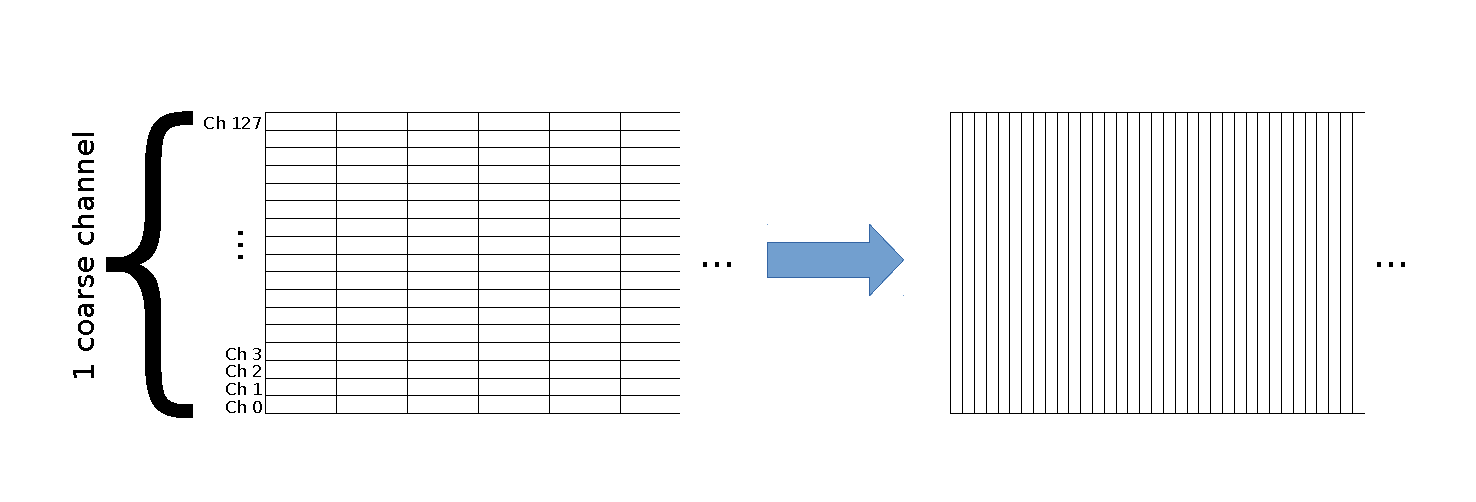
\includegraphics[scale=0.6]{images/pfb_fig1.pdf}
    \vspace{-1cm}
    \caption{A schematic of the data transformation that takes place under the PFB inversion algorithm. On the left are the fine-channelised time samples, sampled at $10\,$kHz. On the right is a single channel, sampled at $1.28\,$MHz, in which each time sample is a weighted sum of a block of original $10\,$kHz time samples.}
    \label{fig:schematic}
\end{figure}

{\bf Each resynthesised time sample is simply a weighted sum of a block of fine channel samples}, and the pairing of samples and weights for a given output time sample is described below.
The weights are derived from the filter coefficients that were used in the (forward) PFB.
These filter coefficients, in their original form, are a fixed set of 1536 ($= 12 \times 128$) real numbers, shown in Fig. \ref{fig:filter_coeffs}.
\begin{figure}[!b]
    \centering
    \includegraphics[scale=0.45]{images/filter_coeffs.png}
    \caption{The PFB filter coefficients, retrieved from \url{http://mwa-lfd.haystack.mit.edu/twiki/bin/view/Main/Finepfb}. The vertical lines divide the coefficients up into 12 sets (or ``taps'') of 128 coefficients each.}
    \label{fig:filter_coeffs}
\end{figure}
In order to keep the magnitudes of the resulting numbers small (for packing into 8-bit integers for the VDIF format), we scale the filter coefficients down by the (arbitrary) factor $1.2 \times 10^{5}$.
This number was chosen to normalise the maximum coefficient value to approximately $1$.

Using the 1536 filter coefficients, we now form a 2D array ($128 \times 1536$) of weights as follows.
The filter coefficients ($f$) are copied into each row, and each element $(i,j)$ is multiplied with a complex number with unit length and phase $\phi_{ij}$.
That is, the weights array is
\begin{equation}
    w_{ij} = f_j e^{\phi_{ij}},
\end{equation}
where
\begin{equation}
    \phi_{ij} = \frac{-2\pi(i-i_c)j}{128},
\end{equation}
and where $i_c$ is the row number associated with the central fine channel, corresponding to the ``DC'' bin (in our case, $i_c = 64$, remembering that channel numbers start at $0$).
The result is a complex-valued 2D array whose magnitudes and phases are plotted in Fig. \ref{fig:weights}.
\begin{figure}[!b]
    \centering
    \includegraphics[scale=0.45]{images/weights_abs.png}
    \includegraphics[scale=0.45]{images/weights_arg.png}
    \caption{The weights array ($128 \times 1536$), generated from the filter coefficients plotted in Fig. \ref{fig:filter_coeffs}. The magnitudes are plotted above, and the phases below.}
    \label{fig:weights}
\end{figure}
Each row of the weights array can be considered as the original filter coefficients multiplied by a {\bf phase ramp} whose slope depends on its proximity to the central fine channel.

The weights array (Fig. \ref{fig:weights}) is multiplied element-wise to an equally sized array formed out of the fine-channelised time samples, as follows.
The time samples are upsampled by inserting 127 zeros between each time step, as illustrated schematically in Fig. \ref{fig:upsample}.
\begin{figure}[!ht]
    \centering
    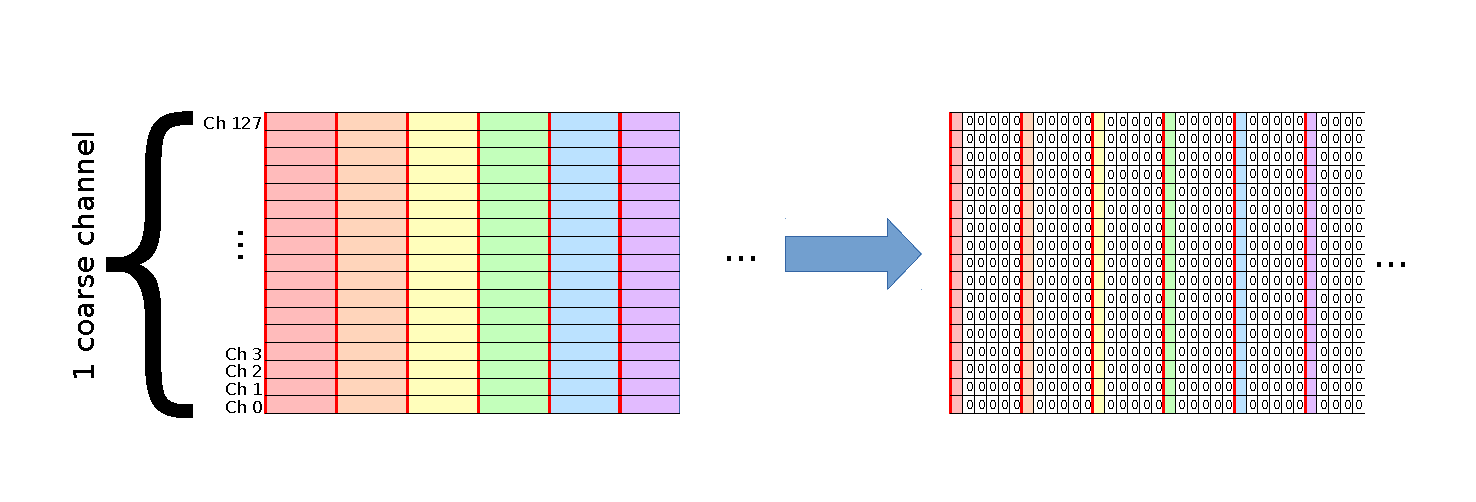
\includegraphics[scale=0.6]{images/pfb_fig2.pdf}
    \vspace{-1cm}
    \caption{A schematic of the process of upsampling the fine-channelised data. In the diagram, the upsampling factor is 6, whereas in this algorithm, the upsampling factor is the same as the number of channels, i.e., 128.}
    \label{fig:upsample}
\end{figure}
The upsampled time samples now form an $128 \times N$ grid, where $N = 128T$, where $T$ is the original number of samples.

The weights array can now be slid horizontally over the upsampled time samples array, shifting across by one sample at a time.
In this algorithm, we have identified the $n$th output time sample (starting, as usual, with $n = 0$) with the slide position in which the rightmost column of the weights array is aligned with the $n$th column of the upsampled time samples array.
In particular, this means that the first sample that makes use of the whole weights array is $n = 1535$, since then the leftmost column is aligned with $n = 0$.
The final value of the $n$th output time sample ($y_n$) is then the sum of the upsampled time samples ($x_n$) multiplied element-by-element with the corresponding weights array slid into the $n$th position:
\begin{equation}
    y_n = \begin{cases}
        0, &\qquad n < 1535, \\[5pt]
              \sum\limits_{i=0}^{(127)} \sum\limits_{j=0}^{(1535)} w_{ij} x_{ij^\prime}, &\qquad \text{otherwise,}
          \end{cases}
    \label{eqn:invertpfb}
\end{equation}
where $j^\prime = j + n - 1536$.

\subsection{Optimisations}

The upsampling of the time samples by a factor of 128 (as shown in Fig. \ref{fig:upsample}) means that almost all (127 out of every 128) of the terms in Eqn. \eqref{eqn:invertpfb} vanish.
Therefore, the algorithm as implemented in \texttt{make\_beam\_small} does not blindly iterate over $i$ and $j$, as the above suggests---instead, only the non-zero terms are considered.
In practise, each output time sample is only the sum of $12 \times 128 = 1536$ non-zero weighted terms, and rather than doing a memory-costly upsampling operation, the indices for the needed terms are calculated as needed.

This works out as follows.
Consider the $n$th output time sample.
The column numbers of the weight matrix that are required for this sample is
\begin{equation}
    j_m = 128(m+1) - (n \mod 128) - 1, \quad \forall m \in \{0,1,\dots,11\}.
\end{equation}
The corresponding columns of the original time samples (i.e. \emph{without} upsampling) are
\begin{equation}
    j_m^\prime = \left\lfloor \frac{n - 1536}{128} \right\rfloor + (m+1), \quad \forall m \in \{0,1,\dots,11\}.
\end{equation}
Thus, Eqn. \eqref{eqn:invertpfb} is actually implemented as
\begin{equation}
    y_n = \begin{cases}
        0, &\qquad n < 1535, \\[5pt]
              \sum\limits_{i=0}^{(127)} \sum\limits_{m=0}^{(11)} w_{ij_m} x_{ij_m^\prime}, &\qquad \text{otherwise,}
          \end{cases}
    \label{eqn:invertpfb_optimised}
\end{equation}
with $j_m$ and $j^\prime_m$ as defined above.

\end{document}
